\documentclass{article}
\usepackage{pgfplots}
\pgfplotsset{compat=1.5}
\begin{document}
\begin{tikzpicture}
\begin{axis}[
title=Inv. cum. normal,
xlabel={$x$},
ylabel={$y$},
]
\addplot [blue] table {invcum.dat};
\end{axis}
\end{tikzpicture}

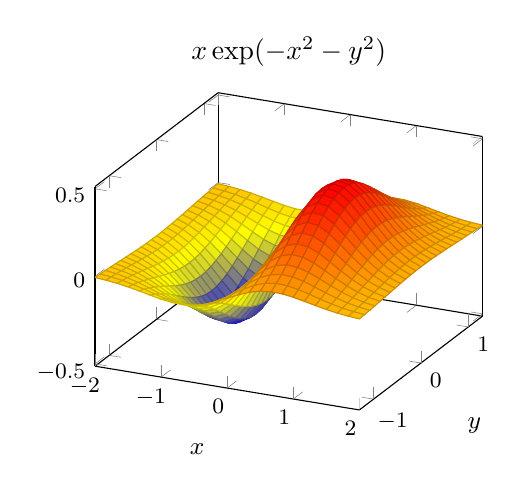
\begin{tikzpicture}
\begin{axis}[
title={$x \exp(-x^2-y^2)$},
xlabel=$x$, ylabel=$y$,
small,
]
\addplot3 [
surf,
domain=-2:2,
domain y=-1.3:1.3,
] {exp(-x^2-y^2)*x};
\end{axis}
\end{tikzpicture}



\end{document}